\chapter{Data Reduction and Analysis}
	\label{cha:Data}
% In Section \ref{sec:}, we lay out the the Southern Sample.
This chapter presents the observations made for this project, of the Southern Sample (as laid out in Section \ref{sec:Sample}) with the VIsable Multi-Object Spectrograph (VIMOS; see Section \ref{sec:VIMOS}). The data-reduction pipeline is laid out in Section \ref{subsec:VIMOSreduction} with a discussion of the data quality, including the artifacts from the VIMOS instrument in Section \ref{subsec:VIMOSartifacts}. Unpublished, archival observations made with the Multi-Unit Spectroscopic Explorer (MUSE) that are also used in this project are described in Section \ref{sec:MUSE}. This includes a discussion of the European Southern Observatory's (ESO's) data-reduction pipeline (Section \ref{subsec:MUSEreduction}). Finally, in Section \ref{sec:analysis}, we describe the data-analysis pipelines, which are used to produce the results presented in Chapters \ref{cha:stellar} and \ref{cha:gas}.  

\section{The VIsable Multi-Object Spectrograph (VIMOS)}
	\label{sec:VIMOS}
	\subsection{The VIMOS Instrument}
		VIMOS is a fibre-fed, multi-purpose spectrograph mounted on Unit Telescope 3 (UT3) on the ESO Very Large Telescope (VLT) in Paranal, Chile \citep{LeFevre2003}. It can operate in a number of configurations: direct imaging, multi-object spectroscopy (MOS) or integral-field spectroscopy (IFS). For this program, VIMOS was used in IFS mode. 

		The integral-field unit (IFU) has a field of view of 40 x 40 spatial pixels (spaxels) with a choice of sampling of 0.67" or 0.33". There are 6 available grisms with varying wavelength ranges and spectral resolutions: low- or high-resolution (LR or HR) red; HR orange; or LR, medium resolution (MR) or HR blue. The observations presented in the following Section were taken using the new (at the time) HR Blue grism with a spatial resolution of 0.67". 

% Find quadrant names - on postit notes on uni screen.
		The field of view of VIMOS is split into 4 quadrants (named in the fits headers, perhaps unhelpful, \_\_\_\_\_\_). The quadrants are run in parallel as independent detectors (it is not possible to use different grisms with different quadrants). Fibres are arranged in a row along the short direction along the charge-coupling device (CCD) detectors, and the light from each fibre is dispersed by the grism in the other direction, giving rise the row-stack spectra (RSS) format of most IFU devices.

		VIMOS has several well known, though not well understood technical issues. These include several low transmission (bad) fibers, strong flexure and large differences in sensitivity across its 4 separate detectors, known as quadrants. These are addressed by a specialist data reduction pipeline as described in Section \ref{subsec:VIMOSreduction} with the a discussion of the resulting data quality in Section \ref{subsec:VIMOSartifacts} (for more detail also see the instrument manual, section 2.8 in current version\footnote{http://www.eso.org/sci/facilities/paranal/instruments/vimos/doc.html}).

	\subsection{Observations with VIMOS}
		As stated above, the observations for this project were taken using the IFS mode (with at a spatial resolution of 0.67"), with the blue HR grism. This grism gives a wavelength range of 3700-5520\,\AA\ at a spectral resolution of 0.71\,\AA\,$\mathrm{pix^{-1}}$. 

		The program of observations (ID: 089.B-0632A) ran in service mode during ESO period 89 and 90. Each object was imaged with a total integration time of $\sim 100$ mins equally spread over three observing blocks (OBs). Each block contained all of the necessary calibration images (3 continuum lamp (flat field) exposures and 1 He and Ne arc lamp exposure for wavelength calibration), as well as two science pointings. In addition, VIMOS provides 5 bias images per night. Flux calibrations were done using public Standards provided by ESO of Feige 110. A summary of the observations is given in Table \ref{tab:observations}.

		


	\subsection{Data Reduction of VIMOS Data}
		\label{subsec:VIMOSreduction}
		The data reduction pipeline was produced using \textsc{Py3D}, a suite of programs based on (the \textsc{python} versions of) those developed for Califa \citep{Sanchez2012, Husemann2013} and later updated for VIMOS by \citet{Husemann2014}. \textsc{Py3D} was provided to us by Husemann (personal correspondence) and is (currently) not publicly available. It  makes use of pixel tables in order to track each pixel through the pipeline, with both spectral and spatial resampling only occurring once. This pipeline accounts for many of the known issues with VIMOS such as bad fibers, strong flexure and cross-talk as well as standard reduction procedures for IFS data. A full outline of the reduction is given here.

		A median master bias is created from the five daily bias frames and subtracted from each raw frame. Known low-transmission (bad) fibres, detected cosmic ray hits and offsets to account for flexure of the instrument due to gravity are taken into account when automatically identifying the fibre positions on the detector. The fibre is then traced along the dispersion axis in the flats. \citet{Husemann2014} finds this to be robust except for a few fibres at the very blue end of the spectrum ($<4300$\,\AA). 

		Since flexure is dependent on position angle of the telescope and rotation of the instrument, the exposures on the source (science exposures) will be affected in a different manner to the flat field exposures. \textsc{Py3D} accounts for the offset of the science exposure to the flat field exposure by tracing the peak fibre position directly on the science exposure at 5 or 6 locations. The offsets are then extrapolated with a second order Legendre polynomial. This corrects for the flexure in the fibre number direction, but flexure also affects the dispersion direction. The effect is estimated by the positions of strong emission lines from the atmosphere (sky lines), however the HR blue only has one sky line at 5199\,\AA, which in many of our science frames was very dim or even not present. This lack of sky lines had previously been an issue with our initial attempt at data reduction using the publicly available \textsc{p3d} program\footnote{http://p3d.sourceforge.net/}. Here the lack of sky lines meant \textsc{p3d} was not able to flux calibrate the quadrants to each other. For this reason (and the lack of accounting for the flexure of VIMOS), we switched to using \textsc{Py3D}. 

		Another issue taken into account by \textsc{Py3D} is cross-talk, where fibres are so densely packed that light from one fibre bleeds into the image of neighboring fibres. The spectra are extracted assuming a Gaussian profile for the cross-dispersion of each fibre with the width fitted for each fibre individually. After this, the spectra are adaptively smoothed to a 3\,\AA\ full-width, half-maximum (FWHM) resolution and resampled.

		Flats are used to correct for the different efficiencies of transmission of each fibre and sensitivities of each CCD pixel (flat-fielding). Each quadrant was then flux calibrated using the observations of the standard star, Feige 110, imaged in each of the 4 quadrants. These observations were reduced in the same way as described above. A mean sky spectrum, built using spectra from the outer regions of the field of view of each quadrant, was subtracted from the science frames. 

		The quadrant were finally combined into a single file, which was converted from the RSS format to a cube (with dimensions of RA, Dec. and wavelength, $\lambda$). Finally, the change in position of the centre of the galaxy due to differential atmospheric refection (DAR) was measured and corrected for. 

		Following on from this, we noted that the cubes where still not fully corrected. A fringe-like pattern was still observable in the spectral direction and quadrants were not calibrated to each other. These were improved by implementing a \textsc{python} version of the ad-hoc corrections given in \citet{Lagerholm2012}. This involves re-normalizing the quadrants to each other by minimizing the difference of the integrated spectra in neighboring fibers along the edge of each quadrant (Q2 was held constant). This was followed by the removal of a fringe-like pattern, by dividing out a smoothed median spectrum from the eight surrounding fibers of any given fiber, over a scale of 150 pixels. These steps mean that the data-cubes will not be perfectly flux-calibrated, however the effect is multiplicative and thus will not effect equivalent width measurements. From comparison the the MUSE data (Section \ref{sec:MUSE}) we estimate flux of the resulting datacubes to be in units of $\sim 10^{-15} \, \mathrm{erg\,s^{-1}\,cm^{-2}}$. 

		The variance spectra is propagated throughout the data reduction pipeline and square-rooted at this point, to be used a noise input in the analysis (Section \ref{sec:analysis})

	\subsection{Data Quality}
		\label{subsec:VIMOSartifacts}













\section{The Multi-Unit Spectroscopic Explorer (MUSE)}
	\label{sec:MUSE}
	\subsection{The MUSE Instrument}
		The Multi-Unit Spectroscopic Explorer (MUSE) is located on UT4 of the VLT. It is comprised of 24 IFU modules with a total field of view of 1 x 1' at spatial sampling of 0.2". It has a spectral range of 4800-9300\,\AA with a resolution of $\approx 2.3$\,\AA\ sampled at 1.25\,\AA\,pix$^{-1}$. MUSE is currently offered with and without adaptive optics (AO) and a narrow-field mode (with an order of magnitude between spatial resolution and sampling) is planned for the future. 
		
	\subsection{MUSE Archival Observations}
		Four of the sample (IC 1459, IC 1531, NGC 1316 and NGC 1399) where found to be in the archive of MUSE data.

		NGC1316 (observed as part of Program ID: 094.B-0298A) and NGC1399 (Program ID: 094.B-0903A) where both observed as mosaics, while IC1459 and IC4296 (both also Program ID: 094.B-0298A) where observed in single pointing. All were observed in the wide-field mode without adaptive optics in service mode during ESO period 94. 

		Every OB in both programs were observed following the standard MUSE calibration plan.

	\subsection{Reducing MUSE Data}
		For this project, the prereduced (known as Phase 3) data products from ESO were used. This means the ESO data reduction pipeline\footnote{http://www.eso.org/sci/software/pipelines/muse/muse-pipe-recipes.html} had already been applied. This was used since the computing resources required to reduce the raw MUSE data may have been prohibitively large.

		The ESO pipeline contains all standard IFU data reduction steps: bias subtraction, flat-fielding of detectors with a continuum lamp exposure, flat-fielding of fibres with twilight exposures, wavelength calibration, flux calibration with standard star observations and sky subtraction. Tiled observations, where present, are combined to give a final mosaic.

		We found that the Phase 3 data products were generally of a sufficient quality for our purposes, except that the sky subtraction in both IC 1459 and IC 426 appear to have over-subtracted large portions of the spectra. This gave the impression of enormous absorption features (often with negative fluxes). To remove this over-subtraction, our own pseudo-sky subtraction routine was developed. The median spectrum was taken from four 20 x 20 spaxel boxes taken from each corner of the observation. After checking that no stellar continuum could be fitted to the spectrum (i.e. there very little light from the galaxy was contaminating our pseudo-sky spectrum), this spectrum was subtracted from each spaxel in the cube. 

		Extra (pseudo-) sky subtractions for NGC 1316 and NGC 1399 were not possible due to mosaic nature of the observations: a sky subtraction should to be applied to each observation in the mosaic independently, but since the observations are already combined as part of the automated data reduction, this was not possible. It is also not possible to access data products from part way through the data reduction, such as immediately before the mosaic is produced. Both NGC 1316 and NGC 1399 are not as badly affected as IC 1459 and IC 4296, so they are left uncorrected. 

		Finally, we trimmed all the cubes to the central 30" x 30" (150 x 150 spaxels) in order to both avoid the region used for the pseudo-sky spectrum and to reduce the computing resources required for the spatial binning stage in the data analysis (Section \ref{sec:analysis}). 

		As with the VIMOS data, the variance is propagated throughout the entire data reduction pipeline and is squared-rooted here to used as the noise input in the analysis stage. 
\section{Data Analysis}
	\label{sec:analysis}
	From this point on, the two datasets are treated almost identically. The only difference (other than the different spectral range and resolutions) is that the MUSE datacubes were binned to a higher signal to noise ratio (S/N).



	%
	The entire pipeline summed up is as follows:
	\begin{enumerate}
		\item Spatial binning using Voronoi binning
		\item Find relevant stellar templates by fitting the entire galaxy spectra with all the templates from the Miles library
		\item Estimate redshifts and global line-of-sight velocity dispersion with MCMC routine 
		\item Find best-fitting LOSVD for each individual bin
		\item Use bootstrapping method to estimate uncertainties LOSVD measurements. 
	\end{enumerate}


	\subsection{Spatial Binning}
		\label{subsec:Binning}
		Given that galaxy (the signal) is brightest at the center and fades away radially, while the noise, which is assumed to be Poisson dominated scales as the square root of the signal, the S/N will be highest at the center, decreasing with increasing radius. In the outer regions of a galaxy, it becomes too low for to make meaningful fits to the spectra. Because of this we spatially bin to a fixed S/N (increasing a bins size until it reaches the require S/N). This is done using a Voronoi Binning routine\footnote{http://www-astro.physics.ox.ac.uk/~mxc/software/} by \citet{Cappellari2003}. To do this, we defined `signal' and `noise' as the median value of the spectrum and noise spectrum respectively for each spaxel. A S/N of 30 is required for all VIMOS datacubes and 50 for IC 1459 and IC 4296 MUSE datacubes. NGC 1316 and NGC 1399 MUSE datacubes were binned to a S/N of 50 for analysis of the stellar kinematics and 100 for analysis of the emission line kinematics and stellar population. The MUSE datacubes had differing S/N due to the extra (pseudo-)sky subtractions which were applied to IC 1459 and IC 4296. These sky subtractions were successful in removing artifacts from the spectra, allowing us to retain a higher level of spatial information for these two galaxies. The artifacts did not seem to affect the analysis of the stellar kinematics, but did affect the emission line fitting. For this reason we enforced a higher S/N for analysis of the emission lines and were careful subtraction of the emission lines is important (i.e. in analysis of the stellar populations). Figure \ref{fig:egSNR} shows an example of the S/N of the bins. In it, concentric ringed structures can be clearly seen around the center of the galaxy as bins with a S/N just below to target are increased in size by a single spaxel meaning they have a final S/N well over the target.

		% Need to remove bin numbers, galaxy name and redshift and second axis from plot.
		\begin{figure}
			\centering
			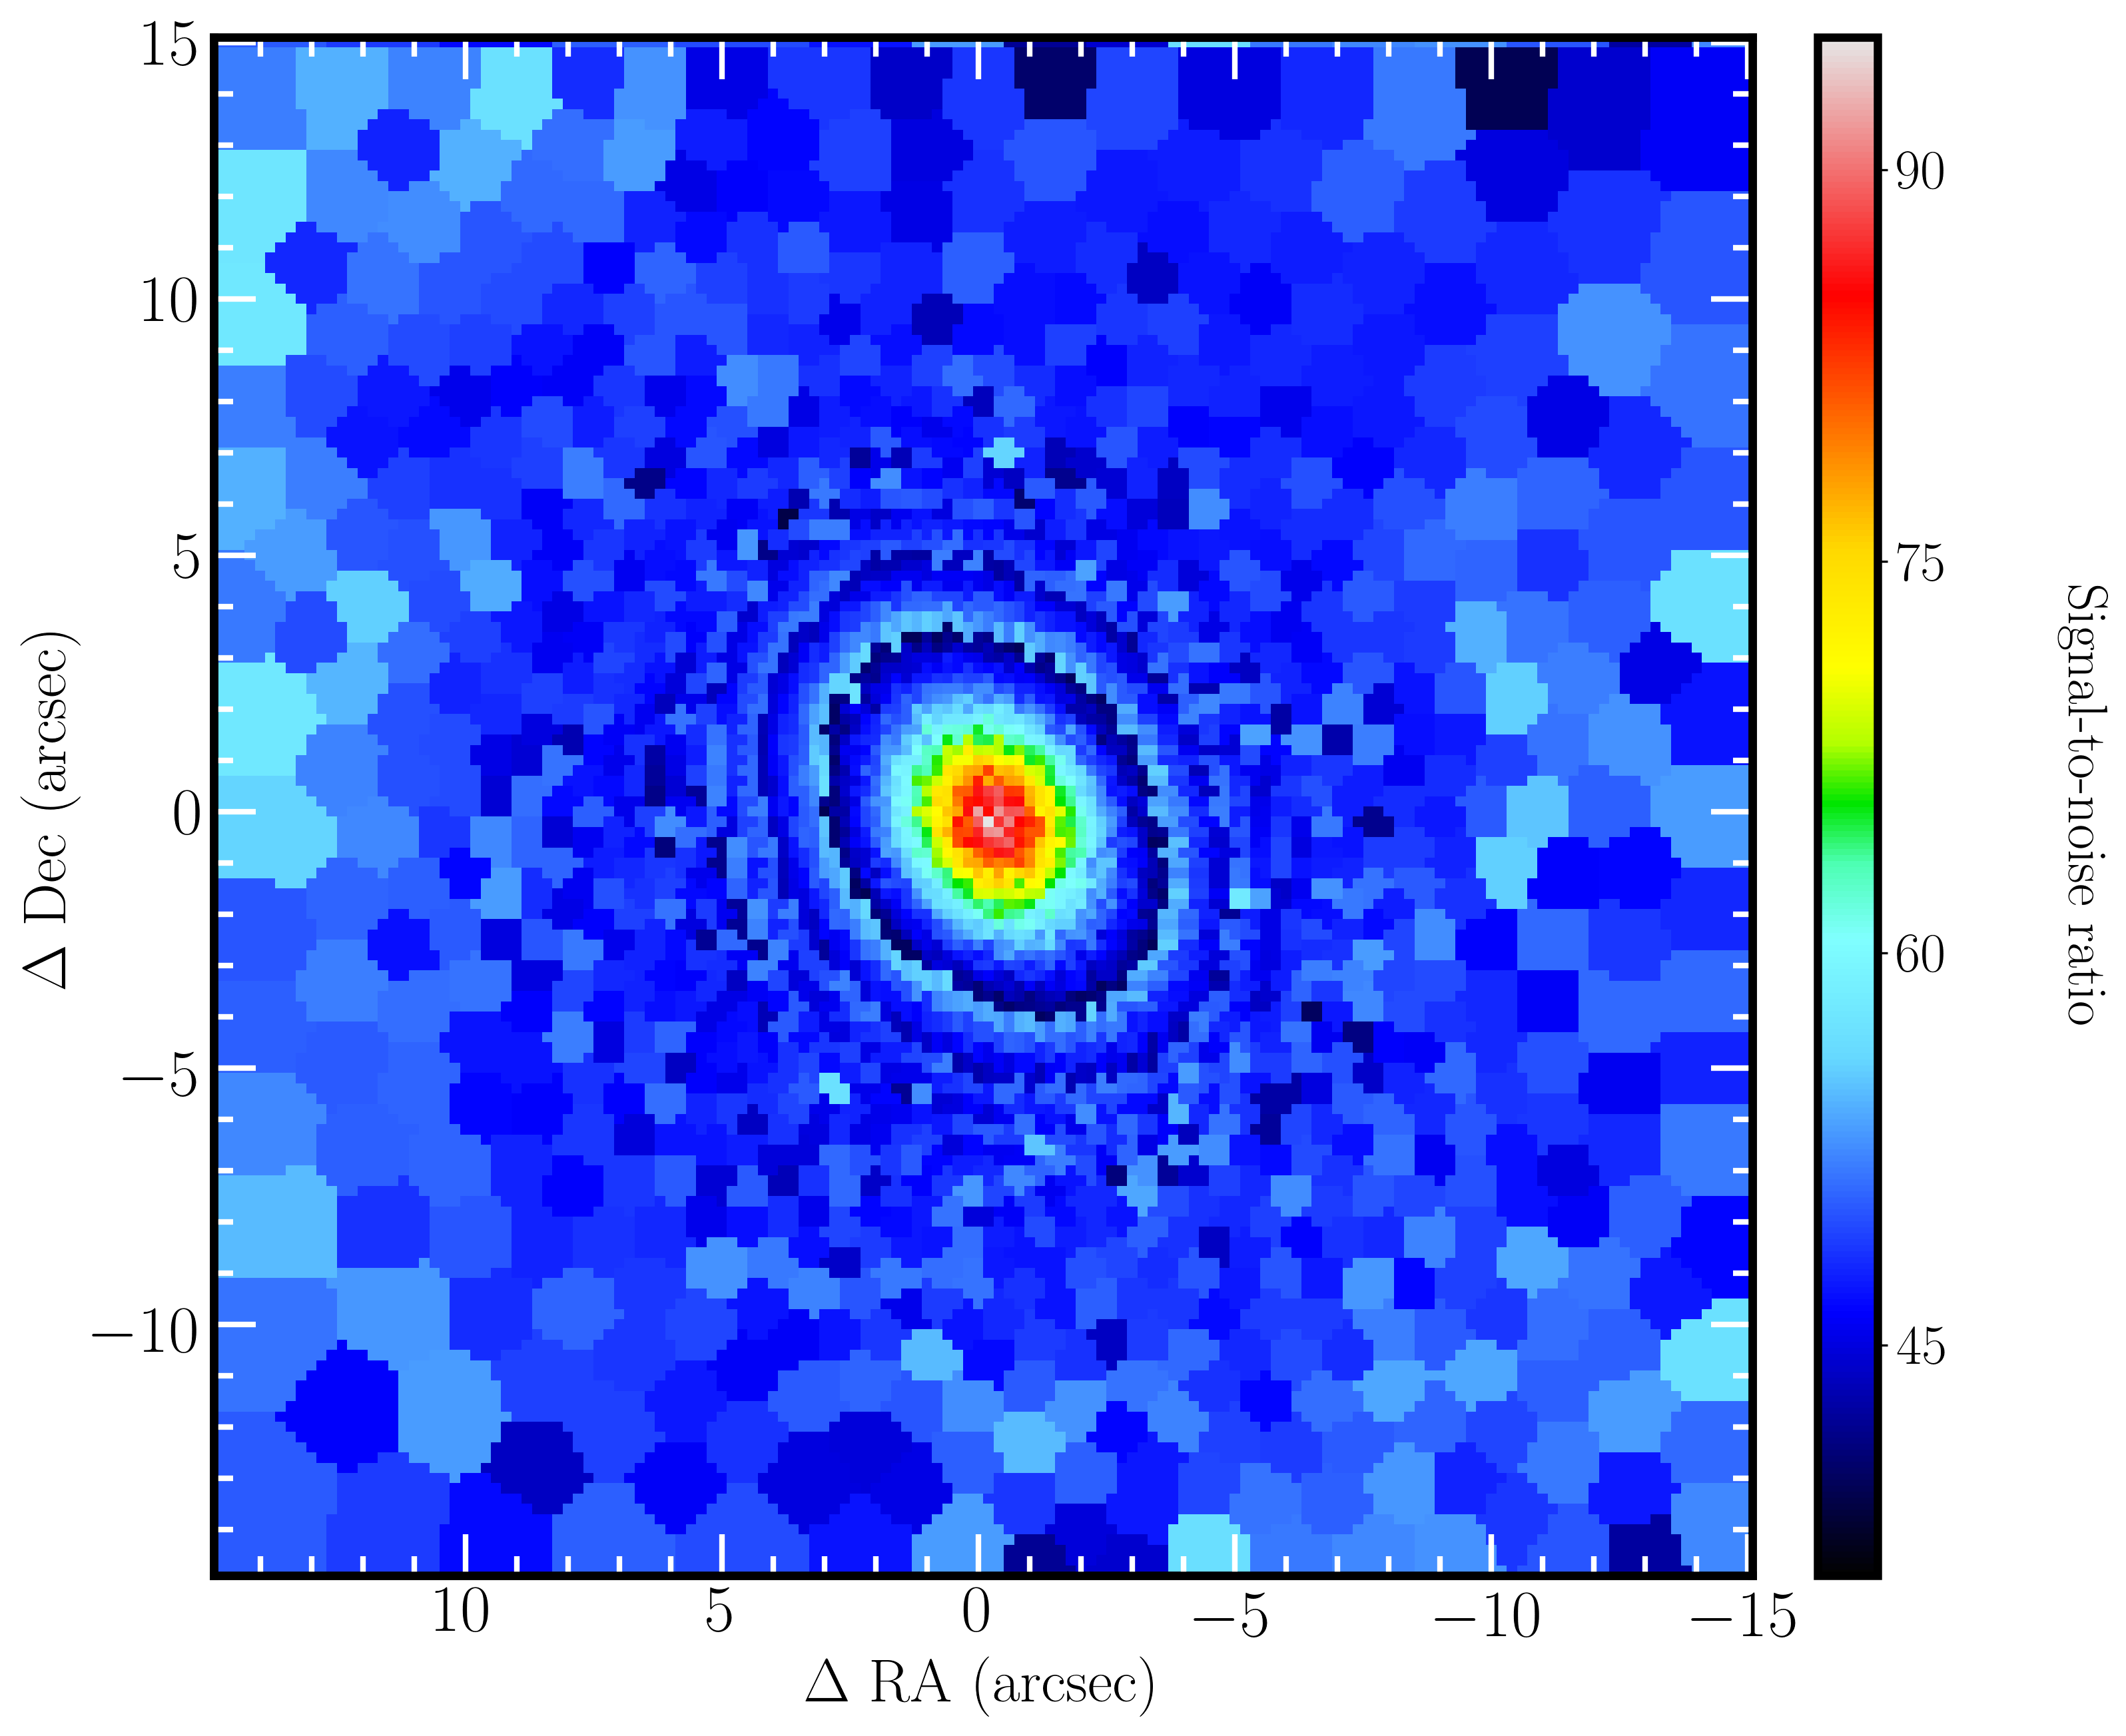
\includegraphics[width=.6\textwidth]{chapter2/egSNR.png}
			\caption[Example S/N map]{The figure shows an example S/N map for the MUSE observation of IC 1459. The flux contours are shown in black.}
			\label{fig:MassRe}
		\end{figure}

	\subsection{Stellar Kinematics}
		\label{subsec:StellarFit}
		Our analysis makes use of the penalized-fitting routine \textsc{pPXF}\footnote{http://www-astro.physics.ox.ac.uk/~mxc/software/} by \citet{Cappellari2004, Cappellari2016a}. This routine finds the best-fitting kinematics by minimizing the reduced chi-squared of a fitted spectrum built from combined empirical stellar templates, convolved with a Gaussian line-of-sight velocity distribution (LOSVD; here parametrised by the mean velocity, $v$, and velocity dispersion, $\sigma$, only). Gaussian templates can also be used to fit emission lines from the interstellar medium (ISM) as independent components (with their own LOSVD). \textsc{pPXF} requires an initial guess for the LOSVD for each component. We using the redshift of the galaxy and $200\,\mathrm{km\,s^{-1}}$ for the initial velocity and velocity dispersion estimates. Finally, Lagrange polynomials can be used to make additive or multiplicative corrections to the continuum level of the fit. A possible sky line at 5199\,\AA\ in the Earth's frame of reference is masked in all fits.

% Find average number of non-zero templates.
		In order to improve the speed of our analysis, we first collapse the datacube spatially to give a global spectra for the galaxy by simply summing across both spatial dimensions at each wavelength. Then the entire Miles stellar library \citep{Sanchez-Blazquez2006, Falcon-Barroso2011a} is used as templates for \textsc{pPXF} to fit. $600\,\mathrm{km\,s^{-1}}$) wide regions around possible emission lines (see Table \ref{tab:EmissionLine}) are masked and a fourth order Lagrange polynomial is used for an additive continuum correction. We use the redshift values from Simbad \citep{Wenger2000} for our initial velocity estimate. For our 14 datacubes (10 VIMOS and 4 MUSE), this step fits an average of \_\_\_\_\_\_ out of 985 templates with a non-zero weighting. Zero-weighted templates are discarded for future analysis of a given datacube. This drastically improves the runtime of \textsc{pPXF} without effecting the quality of the fit.

		% For this fit the redshift from Simbad is used to move the spectra to the rest frame such that an initial guess of the velocity within that frame is 0 km s$^{-1}$. We use a initial guess of the velocity dispersion of 200 km s$^{-1}$ since ETGs have dispersions of around this value and higher. 



		%Regions (600 km s$^-1$ wide) around possible emission lines were masked. Emission lines included were: [OII]3726 , [OII]3729, H$_\delta$, H$_\gamma$, H$_\beta$, [OIII]4959, [OIII]5007, [NI]5199, [NI]5202, [OI]6300, [OI]6364, [NII]6548, [NII]6583, H$_\alpha$, [SII]6716 and [SII]6731. A telluric line at 5199 \AA, seen in some of the VIMOS spectra, was also masked, though the exact location of this depended on the initial redshift 'guess' since the spectrum is moved to the rest frame of the galaxy. For this analysis, we also allowed an additive continuum correction using a fourth order Lagrange polynomial.

		Next we run a Markov chain Monte Carlo (MCMC) routine to find more optimum initial estimates for velocity and velocity dispersion. Of each observation, the initial run is set up in the same way as the previous step (though only using the templates with non-zero weightings). After each run, the fitted velocity and velocity dispersion were used as the initial estimate for \textsc{pPXF}, thus iteratively improving the initial guess with each subsequent run. After the first three reps, the velocity was used to calculate the precise redshift of the galaxy: these are the redshift values quoted in \ref{tab:sample}. After this, small random perturbations to the iterative initial estimates are applied to ensure that the routine converges on a global minimum chi-squared, rather than a local one. 100 repetitions are run, with the mean velocities and velocity dispersions recorded and used as the initial estimates for all subsequent fits in that datacube. 

		Beyond this point, each bin is analyzed independently. Each one is processed through \textsc{pPXF} using only the Miles templates with non-zero weighting from above, using the redshift, additional velocity and dispersion estimates from the last step as the initial required estimate. Again regions around emission lines are masked, and a fourth order additive continuum correction is used. To allow accurate estimation of the propagation of uncertainties in the best-fitting values, a bootstrapping method with 1000 repetitions is used. In each iteration (after the first), random noise, distributed with a Gaussian profile and an amplitude comparable to the noise propagated through the data reduction pipeline, is added to the best-fitting spectrum from the first run. The standard distribution of the fitted parameters from each iteration is used as the quote uncertainty.


	\subsection{Emission-line Kinematics}
		\label{subsec:EmissionFit}
		Fitting emission lines is done in a similar fashion to finding the stellar kinematics. However, in order to combat template mismatches, where emission lines are erroneously fitted to the edges of absorption features that are under represented bu the stellar templates, we follow the recipe set out in \citet{Sarzi2005}. This is a three step process.
		\begin{enumerate}
			\item The region around each emission line's rest frame wavelength is masked, and the stellar spectrum is fitted, then,
			\item the kinematics of the stellar spectrum is fixed to the kinematics found in Step 1. The region around the [\ion{O}{iii}] doublet is then unmasked and fitted. Finally, 
			\item all emission lines are unmasked, but have their kinematics fixed to that found for [\ion{O}{iii}] in Step 2. The emission lines are therefore being fitted with their amplitudes as their only free parameter. 
		\end{enumerate}
		All steps are repeated with the MC method described above to propagate uncertainties and include a tenth order multiplicative Lagrange polynomial to account for continuum emission. 

		The residuals between the best-fitting spectra and the input spectra are smoothed and averaged using a weighted, moving average. This is then summed in quadrature with the noise spectrum to give a combined `residual noise' spectrum. For each fitted emission line, the amplitude (of the fitted line) to the median residual noise (in the region of the emission line) ratio ($A/N$) is used as a detection threshold. As in \citet{Sarzi2005}, for [\ion{O}{iii}], a fit is considered a detection if $(A/N)_{[\text{\ion{O}{iii}}]} \ge 4$; for all other lines, i, except [NI], a detection is recorded if [\ion{O}{iii}] is detected in the same bin and $(A/N)_\mathrm{i} \ge 3$; while a detection of [NI] required a detection of H$_\beta$ and $(A/N)_{[\text{\ion{N}{i}}]} \ge 4$. Emission lines included are given in Table \ref{tab:EmissionLine} along with their rest wavelengths and that of any doublet counterparts (for so-called forbidden lines). 

	 	\begin{table}
	 		\centering
	 	\begin{threeparttable}
	 		\caption{Emission lines included in \textsc{pPXF} fit.}
	 		\label{tab:EmissionLine}
	 		\begin{tabular}{l c c}
	 		\hline
	 		\hline
	 		Line name 		& Rest wavelength (\AA) & Doublet wavelength (\AA) \\
	 		\hline
	 		[\ion{O}{ii}] 	& 3726.03 & 3728.82 \\
	 		H$\delta$ 		& 4101.76 & \\
	 		H$\gamma$ 		& 4340.47 & \\
	 		H$\beta$ 		& 4861.33 & \\
	 		[\ion{O}{iii}] 	& 4958.92 & 5006.84 \\
	 		[\ion{N}{i}] 	& 5199.36 & 5201.86 \\
	 		[\ion{O}{i}] 	& 6300.30 & 6363.67 \\
	 		[\ion{N}{ii}] 	& 6548.03 & 6583.41 \\
	 		H$\alpha$ 		& 6562.30 &\\
	 		[\ion{S}{ii}] 	& 6716.47 & 6730.85 \\
	 		\hline
	 		\hline
	 		\end{tabular}
	 	\end{threeparttable}
	 	\end{table}




	 \subsection{Stellar Populations}
	 	\label{subsec:PopFit}



